% Chapter Template

\chapter{Resultados} % Main chapter title

\label{Chapter4} % Change X to a consecutive number; for referencing this chapter elsewhere, use \ref{ChapterX}

\lhead{Capítulo 4. \emph{Resultados}} % Change X to a consecutive number; this is for the header on each page - perhaps a shortened title

\section{Resultados de Rendimiento}

\subsection{Tiempos de Exportación}
A continuación se analizan los tiempos de exportación de Blender al formato MRR que ofrece \studio

\subsubsection{Exportación de Objetos Simples}
\begin{table}[h!]
\centering
\begin{tabular}{|l|l|l|l|l|l|}
\hline
Nº de objetos & 5  & 10 & 20 & 50 & 80 \\ \hline
Segundos           & 0.2322 & 0.3515 & 0.6927 & 2.0739 & 3.1122 \\ \hline
\end{tabular}
\caption[Exportación de Objetos Simples]{Exportación de Objetos Simples}
\label{ll:expsimple}
\end{table}

\subsubsection{Exportación de Objetos Complejos}
\begin{table}[h!]
\centering
\begin{tabular}{|l|l|l|l|}
\hline
Nº de objetos & 5  & 10 & 20 \\ \hline
Segundos           & 29.30 & 114.48 & 364.35 \\ \hline
\end{tabular}
\caption[Exportación de Objetos Simples]{Exportación de Objetos Simples}
\label{ll:expsimple}
\end{table}

Por excesos en tiempo de computación no ha sido posible obtener datos con más de 20 objetos en la escena

\subsection{Tiempos de Carga}
A continuación se ofrecen los tiempos de carga que ofrece \robotto al cargar en memoria un fichero MRR

\subsubsection{Carga de Objetos Simples}
\begin{table}[h!]
\centering
\begin{tabular}{|l|l|l|l|l|l|}
\hline
Nº de objetos & 5  & 10 & 20 & 50 & 80 \\ \hline
Milisegundos           & 84 & 266 & 238 & 483 & 757 \\ \hline
\end{tabular}
\caption[Carga de Objetos Simples]{Carga de Objetos Simples}
\label{ll:carsimple}
\end{table}

\subsubsection{Carga de Objetos Complejos}
\begin{table}[h!]
\centering
\begin{tabular}{|l|l|l|l|}
\hline
Nº de objetos & 5  & 10 & 20 \\ \hline
Milisegundos           & 16863 & 56440 & 183373 \\ \hline
\end{tabular}
\caption[Carga de Objetos Complejos]{Exportación de Objetos Complejos}
\label{ll:expcomplejo}
\end{table}



\subsection{Renderizado de Múltiples Objetos Simples}
Se ha decidido comprobar el rendimiento de \robotto al renderizar múltiples objetos simples, es decir, objetos carentes de texturas o animaciones.\\
Todos estos objetos son individuales, es decir, aunque se vean iguales cada uno posee una malla diferente asociada.\\

\begin{table}[h!]
\centering
\begin{tabular}{|l|l|l|l|l|l|}
\hline
Nº de objetos & 5  & 10 & 20 & 50 & 80 \\ \hline
FPS           & 60 & 60 & 59 & 45 & 28 \\ \hline
\end{tabular}
\caption[Renderizado de objetos simples]{Renderizado de objetos simples}
\label{ll:rendersimple}
\end{table}

A continuación se incluye una muestra de capturas de pantalla durante las pruebas de rendimiento:\\

\begin{figure}[h!]
\centering
\subfloat[5 objetos]{
  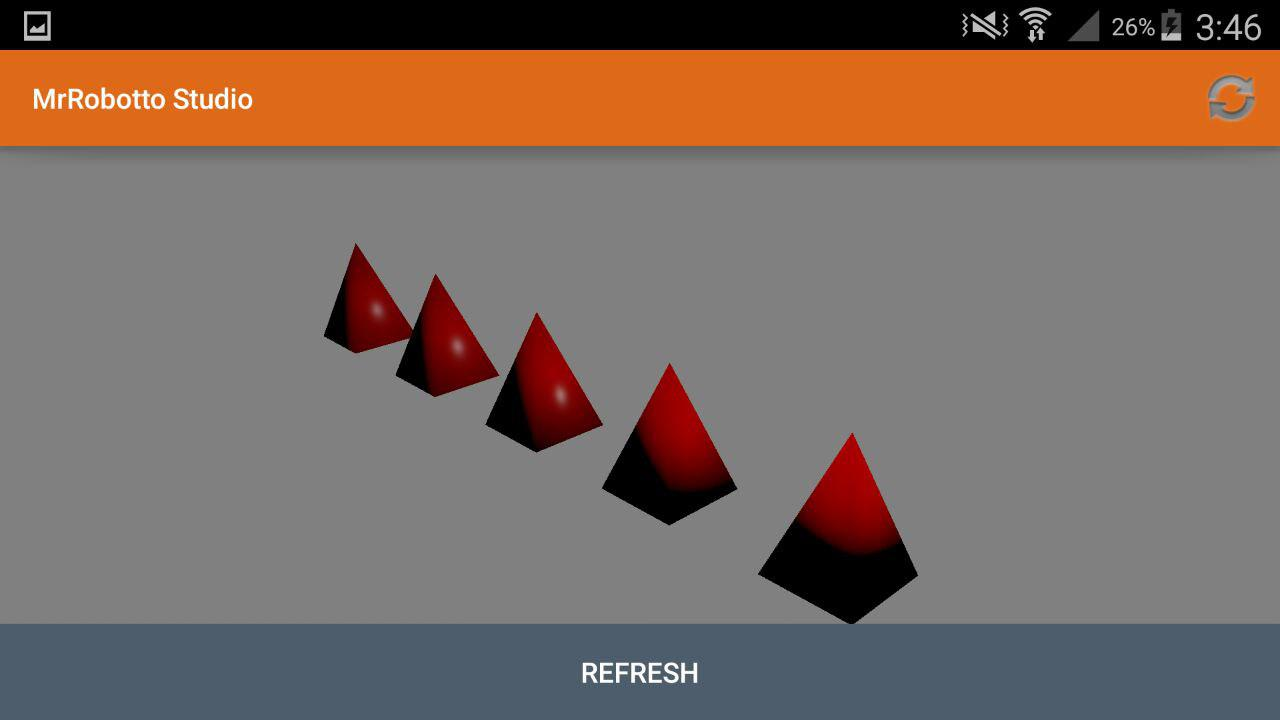
\includegraphics[scale=0.1]{benchmarks/simple/5.jpg}
}
\subfloat[10 objetos]{
  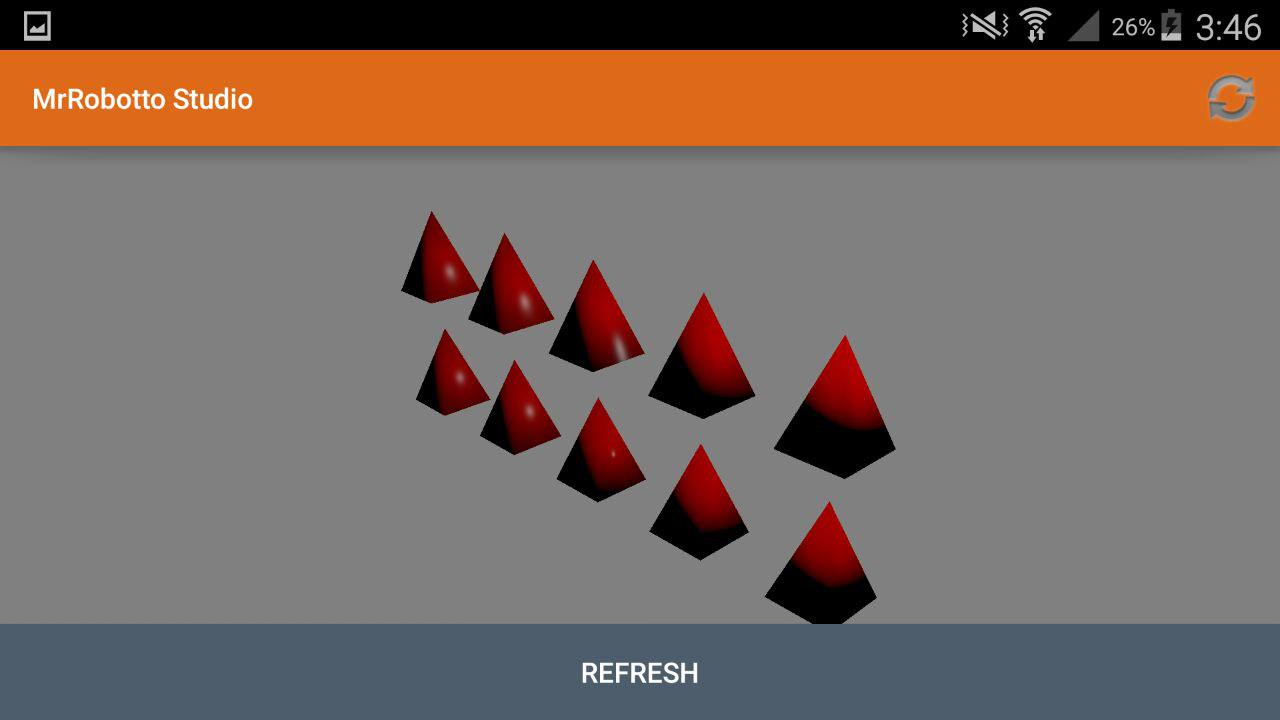
\includegraphics[scale=0.1]{benchmarks/simple/10.jpg}
}
\hspace{0mm}
\subfloat[20 objetos]{
  \includegraphics[scale=0.1]{benchmarks/simple/20.jpg}
}
\subfloat[50 objetos]{
  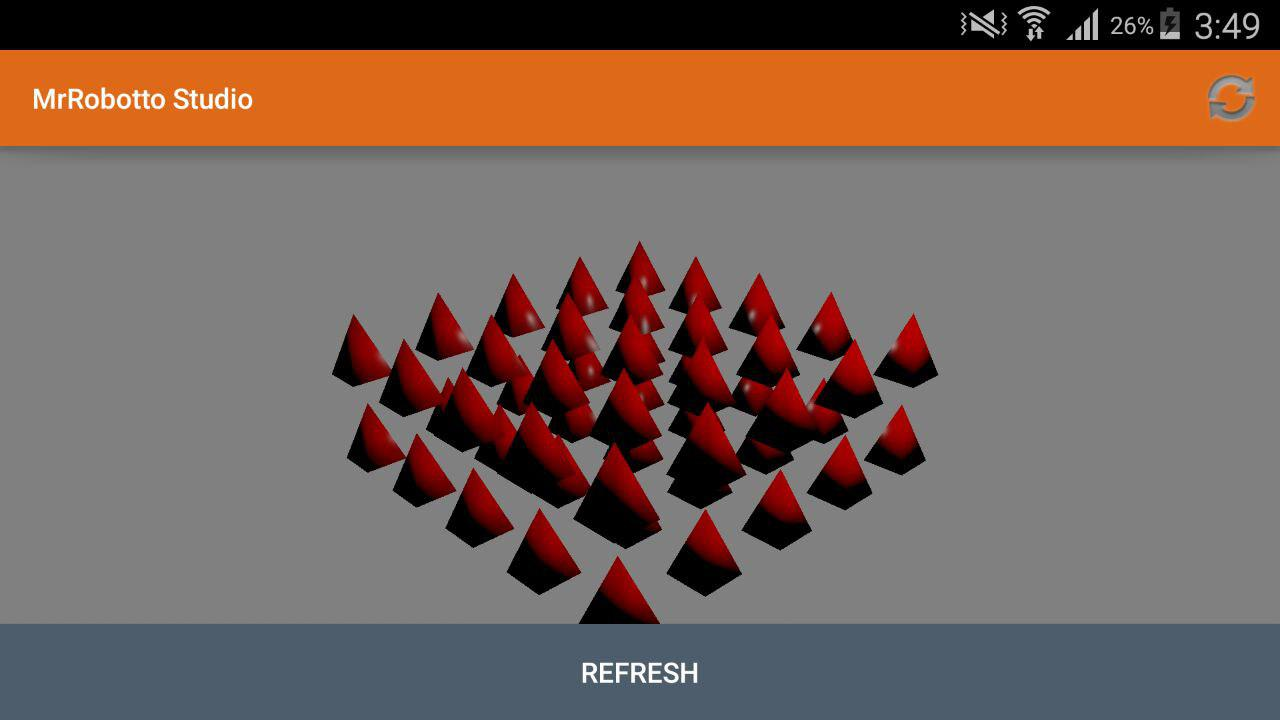
\includegraphics[scale=0.1]{benchmarks/simple/50.jpg}
}
\hspace{0mm}
\subfloat[80 objetos]{
  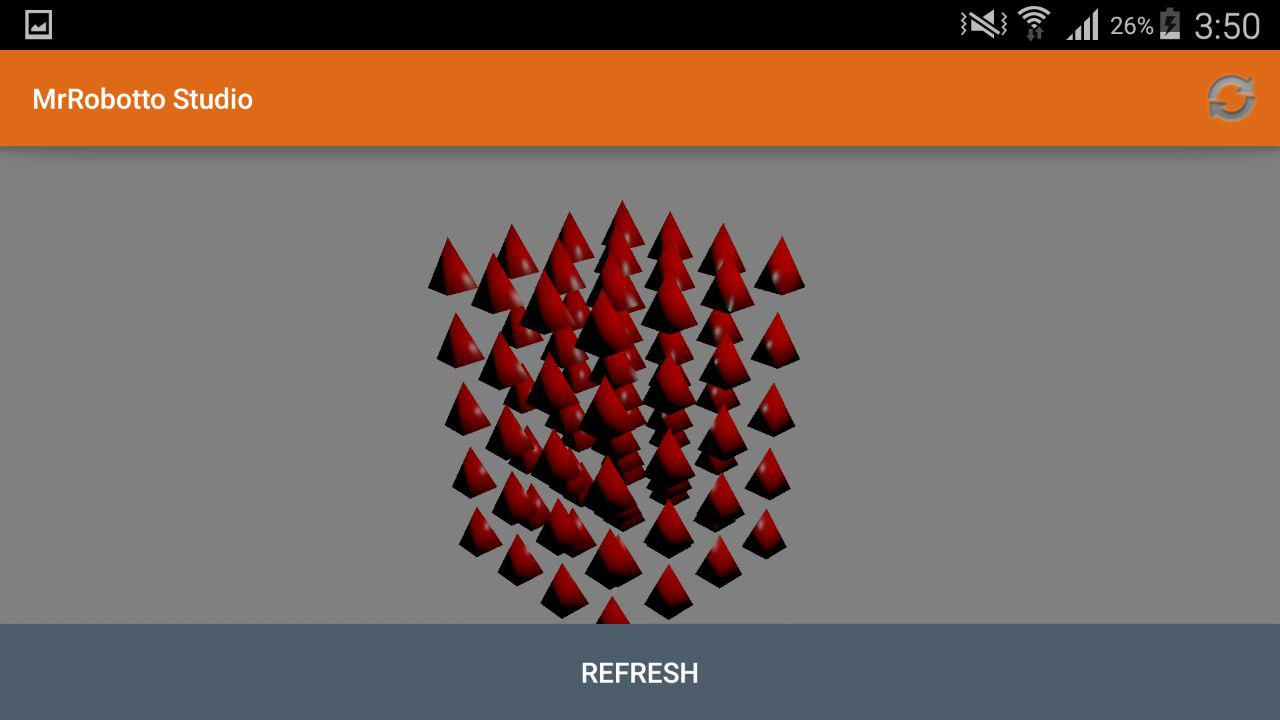
\includegraphics[scale=0.1]{benchmarks/simple/80.jpg}
}
\caption[Renderizado de objetos simples]{Renderizado de objetos simples}
\label{fig:benchmarksimple}
\end{figure}

\subsection{Renderizado de Múltiples Objetos Animados}
Al renderizar múltiples objetos complejos y a su vez animados las pruebas de rendimiento en \robotto han dado como resultado:\\

\begin{table}[h!]
\centering
\begin{tabular}{|l|l|l|l|}
\hline
Nº de objetos & 6  & 12 & 20 \\ \hline
FPS           & 55 & 41 & 20 \\ \hline
\end{tabular}
\caption[Renderizado de objetos complejos animados]{Renderizado de objetos complejos animados}
\label{ll:renderanim}
\end{table}

A continuación se incluye una muestra de capturas de pantalla durante las pruebas de rendimiento:\\

\begin{figure}[h!]
\centering
\subfloat[6 objetos]{
  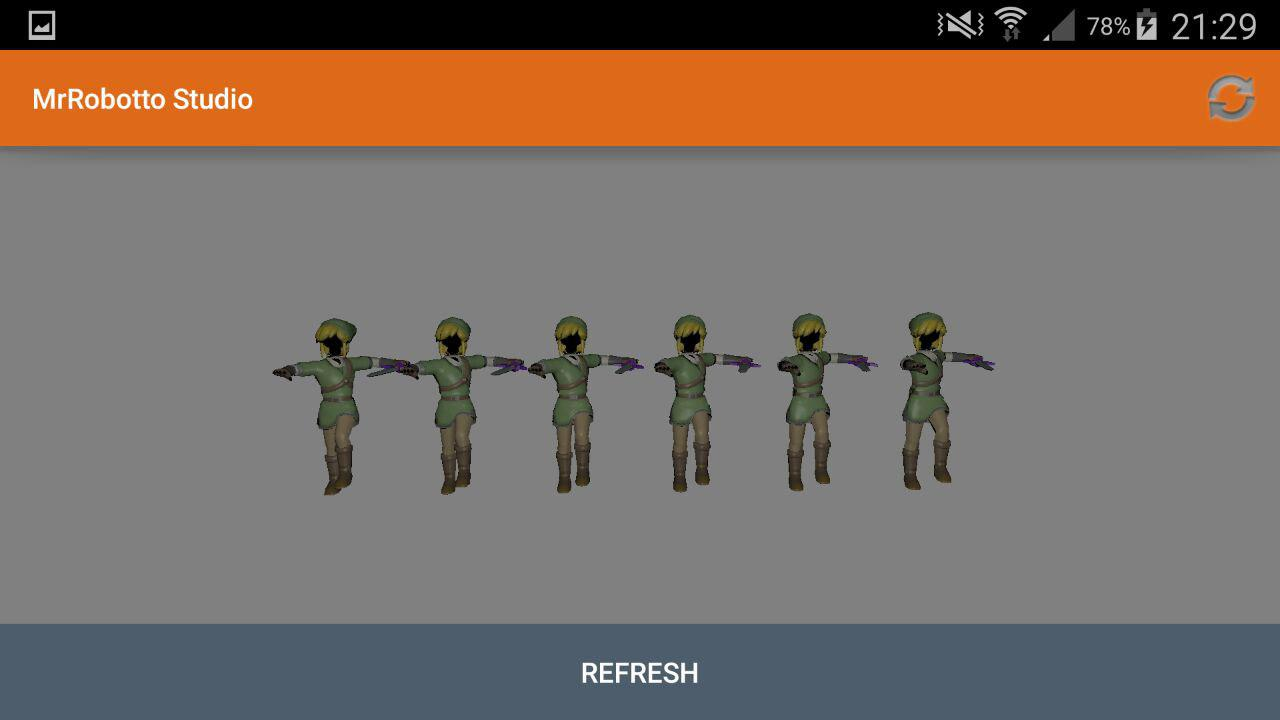
\includegraphics[scale=0.1]{benchmarks/anim/6.jpg}
}
\subfloat[12 objetos]{
  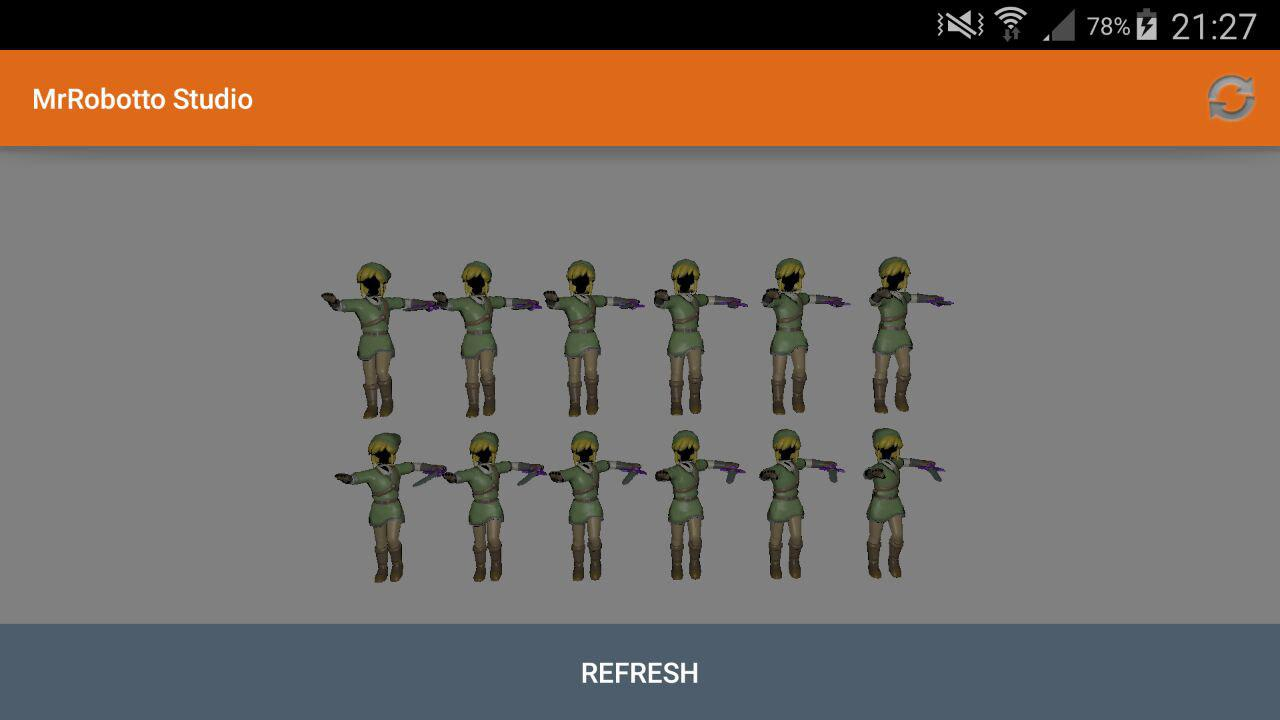
\includegraphics[scale=0.1]{benchmarks/anim/12.jpg}
}
\hspace{0mm}
\subfloat[20 objetos]{
  \includegraphics[scale=0.1]{benchmarks/anim/20.jpg}
}
\caption[Renderizado de objetos simples]{Renderizado de objetos simples}
\label{fig:benchmarksimple}
\end{figure}